%! TEX root = part5.tex
% the main TeX file which is intended to compile, :VimtexReload after adjustment
% :h vimtex-tex-root
\documentclass[../main.tex]{subfiles}
% \includeonlyframes{current}
% \setbeameroption{hide notes} % Only slides
% \setbeameroption{show only notes} % Only notes
\setbeameroption{show notes on second screen=right} % Both

\begin{document}

\begin{frame}[mytitle=standard,c,mybg=addlightbg,light]
	\frametitle{Tugas Kelas(Lanjutan)}

	\txt{digiPH_leaf}{digiPH_white}{Perbaiki maket dari pondasi hingga balok berdasarkan denah yang tersedia}
	\scriptsize Kelompok

	\normalsize	Perbaiki Gambar Kerja \huge Rencana Sloof \normalsize dan \huge Rencana Kolom \normalsize
	Individu
\end{frame}

\end{frame}

\begin{frame}[mytitle=standard,t,mybg=bglight3,light]
	\frametitle{Kayu dan Bambu}
	\begin{itemize}
		\item Kayu dan bambu adalah material alami yang banyak digunakan dalam konstruksi
		\item Kayu:
		      \begin{itemize}
			      \item Kayu keras (jati, mahoni)
			      \item Kayu lunak (pinus, cemara)
		      \end{itemize}
		\item Bambu:
		      \begin{itemize}
			      \item Termasuk keluarga rumput
			      \item Contoh: bambu petung, bambu hitam
		      \end{itemize}
		\item Bambu lebih cepat tumbuh → lebih berkelanjutan
	\end{itemize}
\end{frame}

\begin{frame}[mytitle=standard,t,mycolor=digiPH_white,light]\frametitle{Perbandingan Kayu dan Bambu}
	\begin{itemize}
		\item Bambu:
		      \begin{itemize}
			      \item Tumbuh cepat dan ramah lingkungan
			      \item Kuat tarik tinggi dan fleksibel
			      \item Rentan terhadap kelembapan dan hama
		      \end{itemize}
		\item Kayu:
		      \begin{itemize}
			      \item Tahan lama dan estetis
			      \item Mudah diolah
			      \item Waktu tumbuh lama → risiko deforestasi
		      \end{itemize}
	\end{itemize}
\end{frame}

\begin{frame}[mytitle=standard,t,mycolor=digiPH_gray,light]
	\frametitle{Bambu dan Kayu dalam Konstruksi}
	\begin{itemize}
		\item Digunakan untuk:
		      \begin{itemize}
			      \item Struktur bangunan
			      \item Furniture
			      \item Kerajinan
		      \end{itemize}
		\item Bambu:
		      \begin{itemize}
			      \item Cocok untuk daerah gempa
			      \item Fleksibel dan ringan
		      \end{itemize}
		\item Kayu:
		      \begin{itemize}
			      \item Cocok untuk elemen struktural utama
		      \end{itemize}
	\end{itemize}\end{frame}

\begin{frame}[mytitle=standard,t,mycolor=digiPH_cream,light]\frametitle{Keunggulan Bambu}
	\begin{itemize}
		\item Kekuatan tekan dan lentur baik
		\item Fleksibel terhadap beban gempa
		\item Material sustainable
		\item Dapat menggantikan kayu dalam beberapa aplikasi
	\end{itemize}\end{frame}

\begin{frame}[mytitle=standard,t,mycolor=digiPH_purple,dark]\frametitle{Sistem Sambungan Bambu}
	\begin{itemize}
		\item Dua jenis:
		      \begin{itemize}
			      \item Sambungan tradisional
			      \item Sambungan modern
		      \end{itemize}
		\item Perkembangan teknologi meningkatkan kekuatan sambungan
	\end{itemize}\end{frame}

\begin{frame}[mytitle=standard,c,mycolor=digiPH_red,dark]\frametitle{Sambungan Tradisional}
	\begin{itemize}
		\item Sambungan pemanjang
		\item Sambungan ortogonal
		\item Sambungan sudut
		\item Sambungan menerus
		\item Umumnya menggunakan tali (ikat)
		\item Kekurangan:
		      \begin{itemize}
			      \item Kurang kuat
			      \item Kurang efisien secara struktural
		      \end{itemize}
	\end{itemize}\end{frame}


\begin{frame}[mytitle=standard,t,mycolor=digiPH_white,light]
	\frametitle{Sambungan Pemanjang}
	\includegraphics<1>[width=.82\textwidth]{sambpemanjang}
	\includegraphics<2>[width=.86\textwidth]{../figures/sambortogonal.jpeg}
	\includegraphics<3>[width=.86\textwidth]{../figures/sambsudut.jpeg}
	\includegraphics<4>[width=.86\textwidth]{../figures/sambmenerus.jpeg}
	\includegraphics<5>[width=.86\textwidth]{../figures/sambplat.jpeg}
	\includegraphics<6>[width=.86\textwidth]{../figures/samb_baut.jpeg}
\end{frame}


\begin{frame}[mytitle=standard,t,mybg=bglight1,light]\frametitle{Sambungan Modern}
	\begin{itemize}
		\item Menggunakan:
		      \begin{itemize}
			      \item Plat kayu
			      \item Mur dan baut
		      \end{itemize}
		\item Kelebihan:
		      \begin{itemize}
			      \item Lebih kuat
			      \item Lebih stabil
			      \item Lebih presisi
		      \end{itemize}
	\end{itemize}\end{frame}

\begin{frame}[mytitle=standard,t,mybg=bglight3,light]
	\frametitle{Struktur Kayu}
	\begin{itemize}
		\item Digunakan pada:
		      \begin{itemize}
			      \item Kuda-kuda atap
			      \item Balok dan kolom
			      \item Jembatan dan perancah
		      \end{itemize}
		\item Perancangan harus berdasarkan:
		      \begin{itemize}
			      \item Perhitungan struktur
			      \item Prinsip mekanika
			      \item Standar dan peraturan
		      \end{itemize}
	\end{itemize}\end{frame}

\begin{frame}[mytitle=standard,t,mycolor=digiPH_uniblue,light]\frametitle{Pembebanan Struktur Kayu}
	\begin{itemize}
		\item Beban tetap (>3 bulan)
		      \begin{itemize}
			      \item Berat sendiri, tekanan tanah, air
		      \end{itemize}
		\item Beban sementara (<3 bulan)
		      \begin{itemize}
			      \item Beban manusia, aktivitas ruang
		      \end{itemize}
		\item Beban khusus:
		      \begin{itemize}
			      \item Suhu, gempa, gaya dinamis
		      \end{itemize}
	\end{itemize}\end{frame}

\begin{frame}[mytitle=standard,t,mycolor=digiPH_uniblue,light]\frametitle{Ketentuan PKKI}
	\begin{itemize}
		\item Ukuran minimum penampang:
		      \begin{itemize}
			      \item Minimal sisi 4 cm
			      \item Luas minimal 32 cm$^2$
		      \end{itemize}
		\item Perlemahan harus diperhitungkan pada:
		      \begin{itemize}
			      \item Tarik
			      \item Lentur
		      \end{itemize}
		\item Tidak perlu pada tekan (jika lubang tertutup)
	\end{itemize}\end{frame}

\begin{frame}[mytitle=standard,t,mybg=bglight3,light]\frametitle{Lendutan Maksimum}
	\begin{itemize}
		\item Struktur terlindung: L/300
		\item Struktur tidak terlindung: L/400
		\item Kuda-kuda: L/200
		\item Rangka batang: L/700
	\end{itemize}\end{frame}

\begin{frame}[mytitle=standard,t,mycolor=digiPH_white,light]\frametitle{Modulus Elastis Kayu}
	\begin{center}
		\begin{itemize}
			\item Kelas I : 125.000 kg/cm$^2$
			\item Kelas II : 100.000 kg/cm$^2$
			\item Kelas III : 80.000 kg/cm$^2$
			\item Kelas IV : 60.000 kg/cm$^2$
		\end{itemize}
	\end{center}
\end{frame}

\begin{frame}[mytitle=standard,c,mybg=bglight2,light]\frametitle{Desain Ramah Lingkungan}
	\begin{itemize}
		\item Material alami → efisiensi energi
		\item Mengurangi dampak lingkungan
		\item Bambu lebih unggul dalam keberlanjutan
		\item Kayu unggul dalam kekuatan dan daya tahan
	\end{itemize}\end{frame}

\begin{frame}[mytitle=standard,t,mycolor=digiPH_cream,light]
	\frametitle{Studi Kasus: Green Village Bali}
	\begin{itemize}
		\item Menggunakan bambu sebagai struktur utama
		\item Ramah lingkungan dan berkelanjutan
		\item Memanfaatkan energi terbarukan
		\item Desain menyatu dengan alam
	\end{itemize}
\end{frame}


\begin{frame}[mytitle=standard,t,mycolor=digiPH_white,light]
	\frametitle{Studi Kasus: Green Village Bali}
	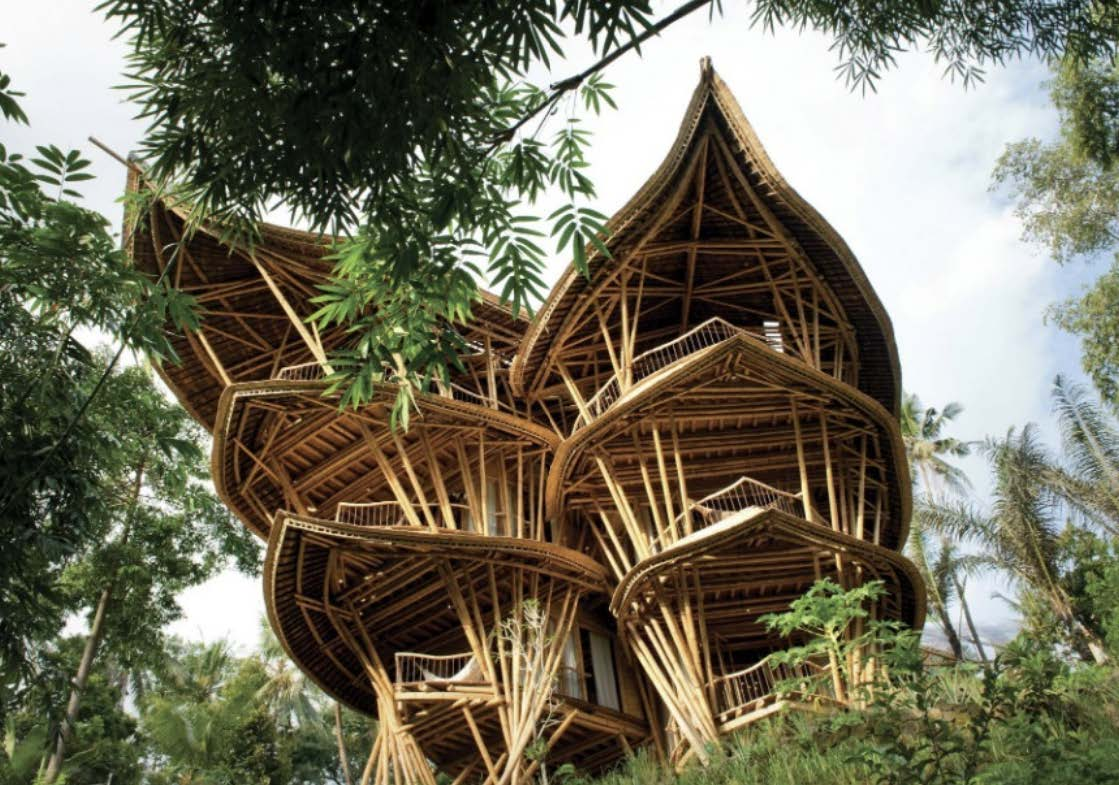
\includegraphics[width=.82\textwidth]{../figures/greenvillage.jpeg}
\end{frame}

\begin{frame}[mytitle=standard,t,mycolor=digiPH_cream,light]
	\frametitle{Studi Kasus: Rumah Adat Toraja}
	\begin{itemize}
		\item Menggunakan kayu lokal (ulin)
		\item Tahan lama dan kuat
		\item Teknik konstruksi tradisional
		\item Ventilasi alami dan adaptif terhadap lingkungan
	\end{itemize}\end{frame}

\begin{frame}[mytitle=standard,t,mycolor=digiPH_white,light]
	\frametitle{Studi Kasus: Rumah Adat Toraja}
	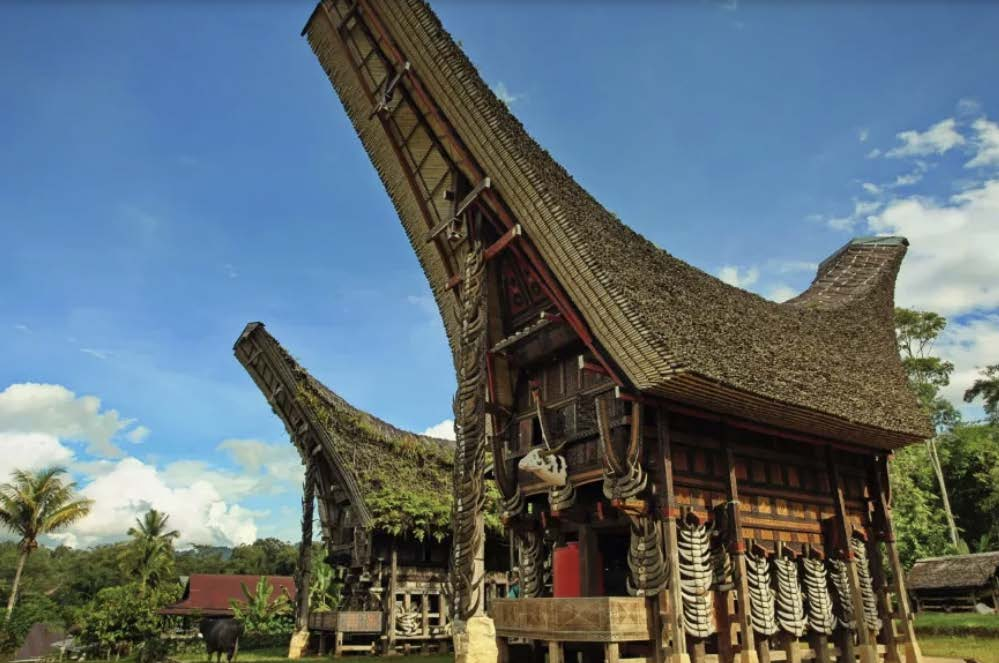
\includegraphics[width=.82\textwidth]{../figures/tongkonan.jpeg}
\end{frame}

\begin{frame}[mytitle=standard,t,mycolor=digiPH_purple,dark]\frametitle{Studi Kasus: Eko-Village}
	\begin{itemize}
		\item Kombinasi bambu dan kayu
		\item Hemat energi dan berkelanjutan
		\item Memanfaatkan sumber daya lokal
		\item Integrasi dengan sistem energi terbarukan
	\end{itemize}\end{frame}


\end{document}
